\section{相似代码搜索}
\label{appendix:sim_code}

代码相似度的主要难点在于智能合约高级语言的结构性特点和逻辑表达形式的多样性。目前学术界对代码相似度的算法大概有下面这些流派:
\begin{itemize}
	\item 字符串编辑距离

把输入query代码和候选源代码都当做文本,利用字符串编辑距离来衡量字符串之间的相似度。编辑距离(Edit Distance)指的两个字符串之间,由一个转成另一个所需的最少编辑操作次数。许可的编辑操作包括将一个字符替换成另一个字符,插入一个字符,删除一个字符。一般来说,编辑距离越小,两个串的相似度越大。这种字符串编辑距离算法既可以用在源代码比较,也可以用在中间语言(intermediate representation),甚至可以用在机器语言中。

为了提高字符串编辑距离算法的健壮性,会对源代码做一些不改变语义的转换,例如:去除空白字符,去除注释,局部变量名统一用'\$'代替,代数表达式的归一化表达等。该算法运算速度快,简洁高效,但是对于复杂程序适应性较差,完全没有考虑到代码的语法和组织结构。

	\item Token序列

Token序列表示法是将输入的源代码通过词汇分析器分析,将源代码转换成Token序列。两个程序的相似度就是Token序列的相似度,可以用最长公共子串,或者相关匹配算法(如后缀树匹配算法)度量程序间的相似程度,这样做可以检测出具有不同句法但却有相似功能的代码段,但该方法在程序相似度度量时隐藏了程序的组织结构。

	\item 抽象语法树(Abstract Syntax Tree,AST)
	
抽象语法树(AST)是对源代码用语法分析后形成的中间表达形式,通过比较子树与其他子树之间的相似程度对程序的相似度进行度量。比较两棵树之间的相似度可以用树的编辑距离算法\cite{zhang1989simple},精确的树编辑距离算法复杂度较大,文献\cite{guha2002approximate}提供了一种近似的快速算法,文献\cite{chilowicz2009syntax}提出对语法树做哈希指纹,使得语法树比较算法可以在海量数据集上进行高效检索。

	\item 程序依赖图(Program Dependency Graph, PDG)

程序依赖图PDG\cite{ferrante1987program}可以表示程序内部数据以及控制依赖关系,能够在语义级别上对程序代码进行分析。相似代码规约成为寻找同构子图,这是NP完全问题,算法复杂度很高,目前只能用一些近似算法。

\end{itemize}

我们认为上述各种算法都在不同维度描述了代码的文本、结构、语法上的相似度。Source Forager\cite{kashyap2017source}提供了一个很好的工程思路,把各种不同维度的相似度指标刻画为不同的特征,每个特征都表征了代码某种方面的相似度衡量,最后用向量的相似度来做总体的相似度衡量,综合了以上各种算法的优点。星云链也借鉴这种思路,实现智能合约的相似搜索。我们把函数作为智能合约代码搜索的基本单位。

表\ref{table:search-similarity}定义了候选的代码相似度特征,我们接下来进一步描述每个特征的定义和它们的相似度计算函数:


\begin{table}[h]
\centering
\begin{threeparttable}[b]
\caption{代码相似度特征族表}
\label{table:search-similarity}
\begin{tabular}{ccc} \toprule
    {Feature-Class} & {Brief Description} \\ \midrule
Type–Operation Coupling & types used and operations performed on the types \\
Skeleton Tree & structure of loops and conditionals \\
Decorated Skeleton Tree & structure of loops, conditionals, and operations \\
3 Graph CFG BFS & CFG subgraphs of size 3, BFS used for generating subgraphs \\
4 Graph CFG BFS & CFG subgraphs of size 4, BFS used for generating subgraphs \\
3 Graph CFG DFS & CFG subgraphs of size 3, DFS used for generating subgraphs \\
4 Graph CFG DFS & CFG subgraphs of size 4, DFS used for generating subgraphs \\
Library Calls & calls made to libraries \\
Type Signature & input types and the return type \\
Local Types & types of local variables \\
Numeric Literals & numeric data constants used \\
String Literals & string data constants used \\
\bottomrule                                                   
\end{tabular}
\end{threeparttable}
\end{table}

\begin{itemize}
	\item \textbf{Type–Operation Coupling:} 该特征是一个二元组集合,二元组包含变量类型,以及变量类型的算符,即(type,operation)对。原生数据类型一般和算术运算符、逻辑运算符以及关系运算符配对,例如($int, \geq$);自定义类型(例如struct)一般和成员函数配对,例如(Bar, .foo)表示数据类型Bar的字段foo被访问。按照这种方法,把一个函数的代码体内部所有变量操作都变成二元组,并且去重以后,就用一个二元组序列体现了这段代码的Type–Operation Coupling特征。我们认为相似功能的代码,也应该具有相似的变量操作集合。但是我们并不关心二元组的先后顺序,所以该特征丢失了代码的逻辑结构信息,只能部分代表代码的特征。
	
	Type–Operation Coupling特征之间的相似度可以由雅克比相似度定义,即如果给定两个集合$S_{1}$和$S_{2}$,雅克比相似度由如下公式定义:
	\begin{equation}
	sim_{Jacc(S_{1},S_{2})}=\frac{\mid S_{1}\bigcap S_{2}\mid}{\mid S_{1}\bigcup S_{2}\mid}
	\end{equation}
	
	\item \textbf{Skeleton Tree:} 基于代码的抽象语法树,但是只保留了循环(for,while,do...while)和条件语句(if...else),其余节点从树中全部移除。我们认为相似功能的代码,应该具有相似的循环和条件语句结构。
	
	Skeleton Tree的相似度计算基于树的编辑距离。定义$d_{r}$为两棵树的预估编辑距离,此距离仅仅由树的大小决定,即:
	\begin{equation}
	d_{r}(T_{1},T{2})=\frac{\mid size(T_{1})-size(T_{2})\mid}{max(size(T_{1}),size(T_{2}))}
	\end{equation}
	假设$D_{T}$是编辑距离的阈值,设定为0.5。我们进一步得到两棵树的近似编辑距离公式:
	\begin{equation}
	d_{t}(T_{1},T{2})=\begin{cases}d_{r}(T_{1},T{2}) & if~d_{r}(T_{1},T{2})\geq D_{T}\\\frac{max\left(\begin{array}{c}ed(pre(T_{1}),~ed(pre(T_{2})),\\ ed(post(T_{1}),~ed(post(T_{2}))\end{array}\right)}{max(size(T_{1}),size(T_{2}))} & otherwise\end{cases}
	\end{equation}
	
	pre(T)代表树的先序遍历序列,post(T)代表树的后序遍历序列,$ed(S_{1},S_{2})$代表序列$S_{1}$和$S_{2}$的编辑距离。Skeleton Tree的相似度可以由以下公式计算:
	\begin{equation}
	sim_{Tree}(T_{1},T{2})=1-d_{t}(T_{1},T{2})
	\end{equation}
	
	\item \textbf{Decorated Skeleton Tree:} 和Skeleton Tree相似,除了循环和分支节点以外,还保留了大部分运算符(例如+,-,<)。但是赋值运算符去除了,因为这些大都是噪音。
	\item \textbf{K-Subgraphs of CFG:} 基于函数的CFG图的k-子图实现。k-子图按如下方法定义:给定CFG图和某节点,我们做广度优先遍历(BFS)或者深度优先遍历(DFS),直至遍历节点数为k,形成的子图为k-子图。如果遍历结束后,节点数不足k,丢弃该子图。遍历CFG图的每个节点,我们可以得到所有的k-子图。对于每个k-子图,我们用$k^{2}$位整数表示,参考图\ref{fig:graph-ex}。所有的k-子图形成了一个整数集合。
	
	\textbf{3 Graph CFG BFS:} k = 3, BFS遍历
	
	\textbf{4 Graph CFG BFS:} k = 4, BFS遍历
	
	\textbf{3 Graph CFG DFS:} k = 3, DFS遍历
	
	\textbf{4 Graph CFG DFS:} k = 4, DFS遍历
	
	相似度可以由广义雅克比相似度公式计算:给定向量$\vec{x}=(x_{1},x_{2},...x_{n})$和$\vec{y}=(y_{1},y_{2},...y_{n})$,广义雅克比相似度定义为
	\begin{equation}
	J(\vec{x},\vec{y})=\frac{\sum_imin(x_{i},y_{i})}{\sum_imax(x_{i},y_{i})}
	\end{equation}
	
	
	\begin{figure}[h]
	\centering
	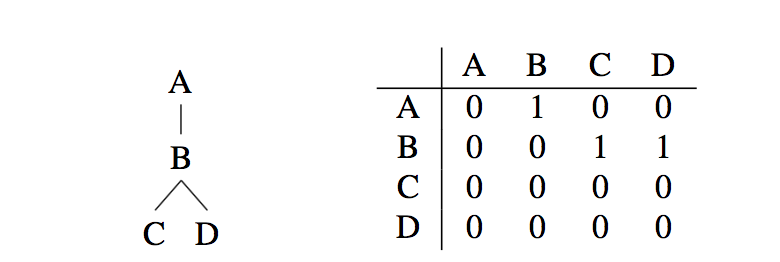
\includegraphics[width=8cm]{./figs/graph-matrix.png}
	\caption{4-graph示例,邻接矩阵的元素为二进制串“0100 0011 0000 0000”, 十进制数为17152}
	\label{fig:graph-ex}
	\end{figure}


	\item \textbf{Library Calls:} 合约中如果发生调用其它库合约,所有库合约的地址也被记录下来,由雅克比相似度公式计算相似度。
	\item \textbf{Type Signature:} 该特征由输入参数类型和返回参数类型组成,由雅克比相似度公式计算相似度。例如对于下面的智能合约代码,函数getBalance的Type Signature特征为向量(address,uint256)。 \\
	
	\begin{figure}[h]
  	\centering
  	\begin{minipage}{.7\linewidth}
	\begin{lstlisting}[frame=single]
contract addressTest {
  function getBalance(address addr) returns (uint) {
  	return addr.balance;
  }
}
	\end{lstlisting}
  	\end{minipage}
	\end{figure}

	
	\item \textbf{Local Types:} 该特征为函数体所有局部变量类型的集合,由雅克比相似度公式计算相似度。
	\item \textbf{Numeric Literals:} 所有数值常量的集合作为Numeric Literals特征,由雅克比相似度公式计算相似度。
	\item \textbf{String Literals:} 所有字符串常量的集合作为String Literals特征,由雅克比相似度公式计算相似度。
\end{itemize}

特征族可扩展,可以方便的把各种新的特征加入进来。基于每个特征都有一个相似度计算,我们把所有特征的相似度做加权和,得到最终的代码相似度:
\begin{equation}
	sim_{combined}(\vec{A},\vec{B})=\frac{\sum_{c=1}^{n_{cl}}sim_{c}(\vec{A_c},~\vec{B_c})\cdot w_{c}}{\sum_{c=1}^{n_{cl}}w_{c}}
\end{equation}

其中,$\vec{A}$和$\vec{B}$是特征向量;$n_{cl}$是特征族个数; $sim_{c}$是针对特征c的相似度计算函数;$\vec{A_c}$和$\vec{B_c}$是特征c的特征向量;$w_{c}$是特征c的权重。权重是可以在大量测试集上,通过机器学习算法训练得到的。
